\section{Da Klinkenberg effect}
In 1941, L.J. Klinkenberg published a paper explainin tha discrepancies dat was found up in experiments when measurin tha permeabilitizzle fo' both liquidz n' gases up in tha same material\cite{klinkenberg1941permeability} yo. His discoveries waz of pimped out importizzle up in tha oil industry
\begin{aquote}{Klinkenberg, 1941}
	It has become common practice up in tha oil industry ta determine tha permeabilitizzle of core material wit dry air; tha shiznit probably employed fo' dis determination be arranged ta operate wit tha outlet of tha sample at or near atmospheric pressure.
\end{aquote}
Dude introduced a linear scalin function $f_c(\text{Kn})$ dat relates what tha fuck his schmoooove ass called tha \textit{apparent permeability} $k_a$ - tha permeabilitizzle measured up in tha lab fo' a gangbangin' fluid wit arbitrary densitizzle - ta tha \textit{absolute permeability} $k_\infty$, tha permeabilitizzle fo' a liquid up in tha high densitizzle limit. Da absolute permeabilitizzle be a cold-ass lil constant dependent only on tha porous medium. Da relation is given as
\begin{align}
	k_a = f_c k_\infty = \left(1 + 4\alpha\frac{\lambda}{L}\right)k_\infty = \left(1 + 4\alpha\text{Kn}\right)k_\infty,
\end{align}
where $L$ is tha diameter of tha channel n' $\alpha\approx 1.15$ is tha no-slip factor up in equation \eqref{eq:noslip_sliplength}. Right back up in yo muthafuckin ass. Since tha mean free path is proportionizzle ta tha inverse pressure, we can write tha scalin function as
\begin{align}
	f_c = \left(1 + \frac{b}{\bar P}\right),
\end{align}
where $b$ be a cold-ass lil constant dependin on tha material. It aint nuthin but tha nick nack patty wack, I still gots tha bigger sack. In figure \ref{fig:klinkenberg_correction_factor}, we peep dat tha Klinkenberg erection factor predicts a permeabilitizzle dat almost fifty times higher fo' a gas up in a material wit $\text{Kn}=10$. Da figure also gotz nuff tha Knudsen erection factor which is discussed up in tha next section. I aint talkin' bout chicken n' gravy biatch. Da Klinkenberg erection factor is derived rockin tha straight-up original gangsta order slip velocitizzle up in equation \eqref{eq:linear_slip_velocity} which aint sufficient fo' high Knudsen numbers as we will peep up in section \ref{sec:results_for_simple_geometries}. Based on higher order slip velocitizzle models, one can derive mo' betta permeabilitizzle erections. 
\begin{figure}[h]
\begin{center}
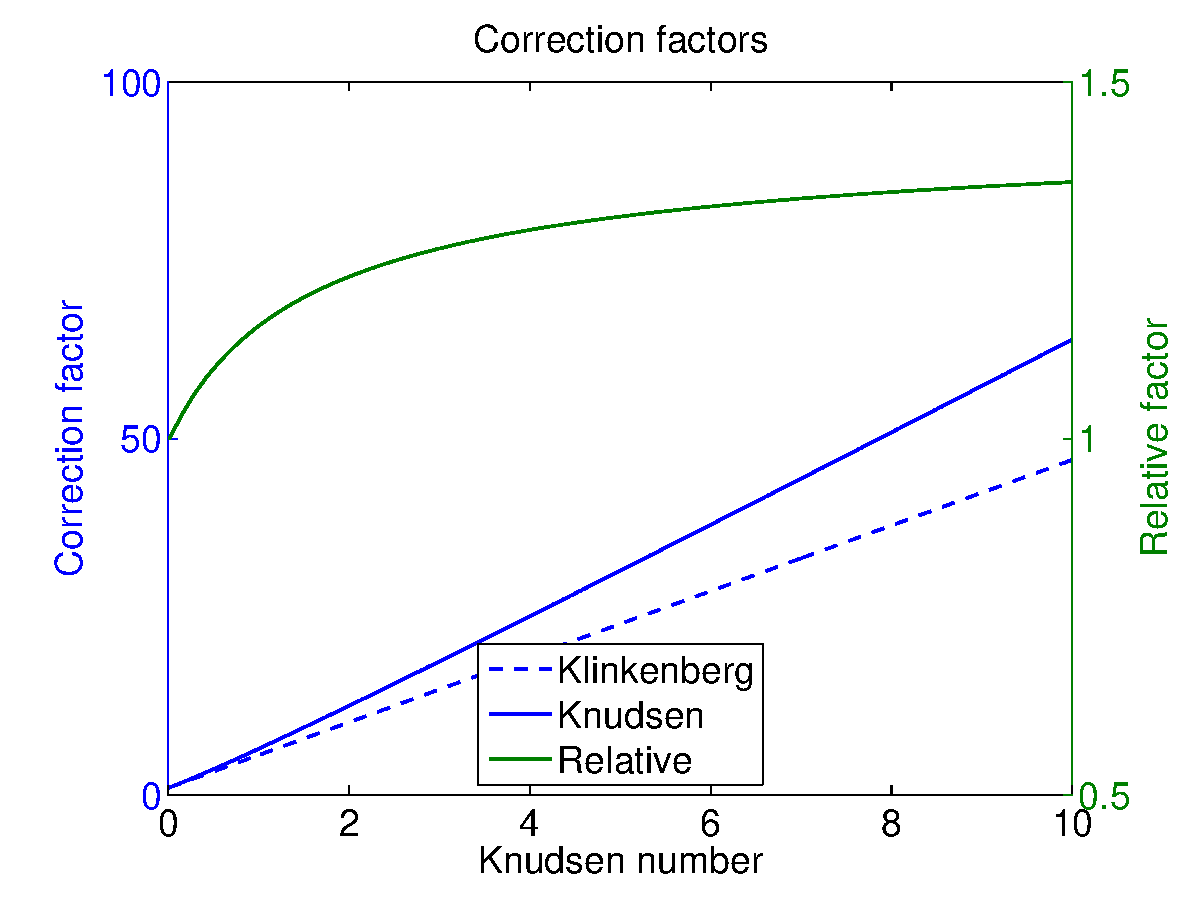
\includegraphics[width=\textwidth, trim=0cm 0cm 0cm 0cm, clip]{figures/klinkenberg.eps}
\end{center}
\caption{A comparison between tha Klinkenberg factor n' tha Knudsen factor shows dat slip velocitizzle leadz ta even higher erections ta tha permeabilitizzle than what tha fuck tha Klinkenberg factor predicts, n' you can put dat on yo' toast. We peep dat up in tha high Knudsen number limit ($\text{Kn}=10$), we can expect a increase of permeabilitizzle by a gangbangin' factor 50 compared ta a liquid or a high densitizzle gas. Da line labeled \textit{Relative} shows tha ratio between tha Knudsen erection n' tha Klinkenberg erection factors.}
\label{fig:klinkenberg_correction_factor}
\end{figure}

\section{Knudsenz erection}
\label{sec:knudsen_correction}
Beskok n' Karniadakis (1999) pimped another erection factor dat uses a second order slip velocitizzle model 
\begin{align}
	\label{eq:knudsen_correction}
	f_c = [1 + \alpha(\text{Kn})\text{Kn}]\left[1 + \frac{4\text{Kn}}{ 1 + \text{Kn}}\right],
\end{align}
where $\alpha(\text{Kn})$ is given as\cite{civan2010effective}
\begin{align}
	\alpha(\text{Kn}) = \frac{\alpha_0}{1 + \frac{A}{\text{Kn}^B}}
\end{align} 
where $A=0.170$, $B=0.4348$, n' $\alpha_0=1.358$. These is fitted parametas based on a big-ass dataset of Loyalka n' Hamoodi (1990). We peep up in figure \ref{fig:klinkenberg_correction_factor} dat tha Knudsen factor predicts approximately 40\% higher erection than tha Klinkenberg factor. Shiiit, dis aint no joke. In chapter \ref{chap:dsmc_results} we will check tha validitizzle of dis erection factor fo' a simple cylinder, n' say shit bout tha practical problems we hook up when studyin flow up in complex geometries where tha system do not simply have one Knudsen number yo, but rather a gangbangin' finger-lickin' distribution of Knudsen numbers.